
\chapter{Das verlassene Expeditionslager}
\noindent\textbf{Akt II -- Szene 3.} Letzte Etappe von Luxor zum Fundort; Abschied von Aziz; freie Erkundung des Lagers.
\begin{meisterinfo}
\textbf{Überblick:} Hier gibt es keine lebenden Expeditionsmitglieder und keine Leichen. Die Ermittler sollen den Ort als überstürzt verlassen erleben, sich mit Material ausrüsten und die Vorgeschichte von Flynn Carlson, Dr. Skorbinsk und Yusuf Hassan vertiefen. Die zuvor gefundene Karte bleibt das zentrale Navigationsmittel im folgenden Dungeon. Aziz ist lebensfroh, kräftig und verlässlich; er betritt die unterirdischen Kammern jedoch unter keinen Umständen. Die vier Zonen des Lagers können in beliebiger Reihenfolge untersucht werden.

\textbf{Zeit:} Später Nachmittag, nach der Reise aus Luxor. Richtzeiten für die Reise bitte als Abenteuerchronologie behandeln, nicht als dokumentierte Fahrpläne.
\end{meisterinfo}
\section{3.1 -- Die letzten Meilen}
\begin{figure}[htbp]\centering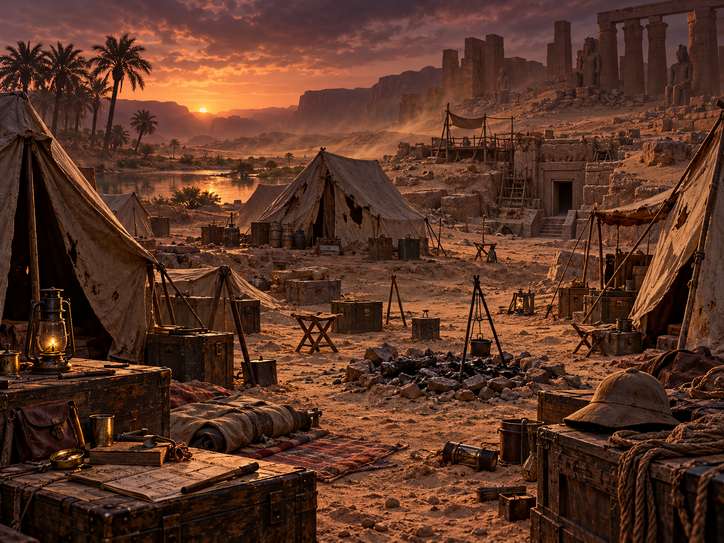
\includegraphics[width=\textwidth]{bilder/lager-verlassen.png}\caption{Das verlassen wirkende Expeditionslager in der ägyptischen Felslandschaft.}\end{figure}
\begin{vorlesetextalle}
Seit dem frühen Morgen seid Ihr unterwegs. Die grünen Felder am Nil liegen weit hinter Euch. Gelbbraune Hügel und ausgedörrte Felsen haben die Landschaft übernommen. Die Sonne steht unerbittlich über den Wagen; selbst das Leder Eures Gepäcks scheint hei\ss{} geworden zu sein. Wenn ein Rad gegen einen Stein schlägt, hallt das Geräusch zwischen den Felswänden wider.

Aziz hat die Fahrt mit Liedern und Geschichten begleitet und sich scherzhaft über die Qualität des Weges beklagt. Doch als der Tross eine niedrige Anhöhe erreicht, verstummt er. Vor Euch liegt eine von Felswänden eingefasste Senke. Ihr erkennt Zelte, verstreute Kisten, aufragende Gestelle und eine dunkle Öffnung im Fels. Kein Mensch bewegt sich zwischen den Zelten.

Aziz hält an. Er mustert die Szene und sagt leise: \glqq{}Da wären wir. Das ist Carlsons Lager. Aber jemand sollte hier sein. Wenigstens die Wächter. Oder der Koch.\grqq{}
\end{vorlesetextalle}
\begin{meisterinfo}
\textbf{Verborgenes Erkennen:} Einige Zelte stehen noch, andere sind eingefallen; Werkzeuge liegen achtlos herum. \textbf{Spurensuche:} Verwaschene Wagen- und Fu\ss{}spuren, aber kein nachvollziehbarer geordneter Abzug. \textbf{Geologie:} An einzelnen Felswänden sind frische Spalten zu erkennen. Kein Wurf ist erforderlich, um das vollständige Fehlen der Menschen zu erkennen.
\end{meisterinfo}
\section{3.2 -- Aziz zieht seine Grenze}
\begin{vorlesetextalle}
Aziz steigt vom Wagen, verschränkt die Arme vor seiner breiten Brust und betrachtet die stillen Zelte. \glqq{}Was für ein Empfang! Nicht einmal jemand, der uns Tee anbietet.\grqq{} Er schmunzelt, aber diesmal klingt das Lachen kürzer als sonst.

\glqq{}Als ich zuletzt hier war, wurde gehämmert, gestritten und gekocht. Jetzt hört man nicht einmal einen Esel. Ich helfe Euch beim Lager, bei der Ausrüstung, bei allem, was ein vernünftiger Mensch tun kann.\grqq{}

Er deutet auf den dunklen Eingang in der Felswand. \glqq{}Aber dort unten hört meine Hilfe auf. Das habe ich Euch versprochen, und ich halte Wort. Ich bin kein Feigling. Ich wei\ss{} nur, wann Mut in Dummheit umschlägt.\grqq{}
\end{vorlesetextalle}
\begin{meisterinfo}
Aziz hilft bei Vorräten, Lampen, Seilen und der Lagererkundung. Er bietet an, bis zum nächsten Morgen zu warten oder später zu einem vereinbarten Termin zurückzukehren. Er lässt sich auch durch beste \emph{Überreden}-Würfe nicht zum Betreten der Grabkammer bewegen. \textbf{Psychologie:} Er ist entschlossen und besorgt, aber nicht panisch. \textbf{Bei Nachfragen:} In der Tiefe hörte er Stimmen vermeintlich längst verschwundener Arbeiter. Aziz darf Kenntnisse über den Weg zum Lager oder dessen Organisation beisteuern; er kennt die jüngsten Ereignisse in den Katakomben nicht.
\end{meisterinfo}
\section{3.3 -- Zwischen Zelten und Kisten}
\begin{vorlesetextalle}
Zwischen den Zelten rascheln lose Planen im Wind. Auf einer Pritsche liegt eine zerknitterte Decke; daneben stehen Stiefel, als sei ihr Besitzer kurz hinausgegangen. Eine Feuerstelle ist erloschen. Im Topf hängen eingetrocknete Essensreste. Schaufeln, Seile und Instrumentenkisten sind liegengelassen worden. Ein Stuhl liegt umgestürzt, eine Tasse steht halb im Sand.

Das Lager sieht nicht ordentlich aufgegeben aus. Es ist, als hätten seine Bewohner ihre Arbeit mitten in einem gewöhnlichen Tag unterbrochen und seien einfach nicht zurückgekommen.
\end{vorlesetextalle}
\subsection{A -- Das Arbeitszelt Flynns}
\begin{vorlesetextalle}
Unter einem ausgeblichenen Zeltdach steht ein Arbeitstisch voller Vermessungsblätter, Bleistifte und Skizzen. Über einer Kiste hängt eine Jacke. Ein Feldstuhl liegt auf der Seite. Die letzte Seite eines offen liegenden Notizhefts ist mit hastiger Schrift gefüllt.
\end{vorlesetextalle}
\begin{meisterinfo}
\textbf{Bibliotheksnutzung oder Verborgenes Erkennen:} Zwischen den Notizen lässt sich ein Eintrag entziffern: \glqq{}Ich habe die Gänge gestern vermessen. Heute stimmen die Entfernungen nicht mehr. Entweder unterlaufen mir Fehler, oder die Anlage verändert sich.\grqq{} Wer die Karte aus Arkham mitbringt, kann Flynns Wegmarken mit den eigenen Beobachtungen vergleichen. Der Eintrag ist auch ohne Probe bei gründlicher Durchsicht zugänglich.
\end{meisterinfo}
\subsection{B -- Das Zelt Dr. Skorbinsks}
\begin{vorlesetextalle}
Bücherkisten, wissenschaftliche Instrumente und unordentliche Blätterstapel füllen das Zelt. Auf mehreren Seiten kehrt dasselbe seltsame Augensymbol wieder. Neben einer Lupe liegen verschmierte Zeichnungen eines handtellergro\ss{}en Steins.
\end{vorlesetextalle}
\begin{meisterinfo}
\textbf{Archäologie:} Viele der Zeichen passen nicht zu bekannter ägyptischer Schrift. \textbf{Okkultismus:} Skorbinsk scheint denselben Gegenstand aus widersprüchlichen Blickrichtungen beschrieben zu haben. \textbf{Aufzeichnungen:} Der Doktor behandelte das Artefakt zunehmend als sein ausschlie\ss{}liches Forschungsobjekt. Seine Person oder das Artefakt selbst befinden sich nicht im Zelt.
\end{meisterinfo}
\subsection{C -- Mannschaftszelte und Kochstelle}
\begin{vorlesetextalle}
Hier stehen einfache Feldbetten und Bündel mit persönlichen Dingen. Auf einer Plane liegen eine Bürste, eine Schale, grobe Arbeitskleidung und eine kleine Stofftasche. Das Feuer ist längst kalt.
\end{vorlesetextalle}
\begin{meisterinfo}
\textbf{Schlüsselbefund:} In der Tasche steht der Name \emph{Yusuf Hassan}. Darin liegen ein Kamm und ein kleiner Messinganhänger mit einer eingravierten Blüte. Ein Gruppenfoto zeigt Yusuf unter Arbeitern der Expedition: die Ermittler erkennen den Mann von der Atlantiküberfahrt. Keine Probe darf diese Wiedererkennung verhindern, falls die Spieler nach Yusuf suchen. \textbf{Psychologie:} Die wenigen zurückgelassenen Habseligkeiten sprechen gegen einen geplanten Aufbruch.
\end{meisterinfo}
\subsection{D -- Das Materiallager}
\begin{vorlesetextalle}
Holzkisten stehen unter einer halb gelösten Plane. Ihr findet Ersatzdochte, Lampenöl, Schaufeln, Hacken, Seile, leere Wasserkanister und ein beschädigtes Vermessungsgerät. Ein Teil des Materials ist brauchbar; anderes hat unter dem Sand gelitten.
\end{vorlesetextalle}
\begin{meisterinfo}
\textbf{Vorbereitung:} Genügend Seile, Wasser, Lampen und einfaches Werkzeug sind verfügbar. \textbf{Mechanische Reparaturen:} Eine defekte Lampe oder ein Vermessungsinstrument kann instand gesetzt werden. \textbf{Spielerinitiative belohnen:} Mehrere Lichtquellen, ein Sicherungsseil und eine markierte Rückroute helfen später bei Sandfalle, Orientierung und Flucht vor dem Dhole. Ressourcen dürfen hier frei geplant werden.
\end{meisterinfo}
\section{3.4 -- Eine Nacht voller Geräusche}
\begin{vorlesetextalle}
Die Sonne ist hinter den Felsen verschwunden. Der Himmel ist schwarz und voller Sterne. Das Feuer knistert, und bei jeder Böe schlagen die Zeltseile gegen ihre Pfosten. Dann dringt aus der Richtung des Eingangs ein dumpfes Rollen, gefolgt von einem tiefen, schleifenden Laut. Unter Euren Fü\ss{}en scheint der Boden kurz zu zittern. Alles wird wieder still.
\end{vorlesetextalle}
\begin{meisterinfo}
\textbf{Horchen oder Geologie:} Die Geräusche erinnern an Bewegungen unter der Erde, sind aber nicht sicher als gewöhnlicher Felssturz erklärbar. Aziz sieht die Ermittler nur ernst an: \glqq{}Ja. Genau das meine ich.\grqq{} Keine erneute Vision. Ein Nachtlager, eine Wache oder ein sofortiger Aufbruch bleiben freie Entscheidungen. \textbf{Abschied:} Aziz verabschiedet sich am Eingang mit kräftigem Händedruck: \glqq{}Wenn Ihr Stimmen hört, ruft nicht gleich zurück. Und kommt wieder heraus, meine Freunde.\grqq{}
\end{meisterinfo}
